% Options for packages loaded elsewhere
\PassOptionsToPackage{unicode}{hyperref}
\PassOptionsToPackage{hyphens}{url}
\PassOptionsToPackage{dvipsnames,svgnames,x11names}{xcolor}
%
\documentclass[
  letterpaper,
  DIV=11,
  numbers=noendperiod]{scrartcl}

\usepackage{amsmath,amssymb}
\usepackage{iftex}
\ifPDFTeX
  \usepackage[T1]{fontenc}
  \usepackage[utf8]{inputenc}
  \usepackage{textcomp} % provide euro and other symbols
\else % if luatex or xetex
  \usepackage{unicode-math}
  \defaultfontfeatures{Scale=MatchLowercase}
  \defaultfontfeatures[\rmfamily]{Ligatures=TeX,Scale=1}
\fi
\usepackage{lmodern}
\ifPDFTeX\else  
    % xetex/luatex font selection
\fi
% Use upquote if available, for straight quotes in verbatim environments
\IfFileExists{upquote.sty}{\usepackage{upquote}}{}
\IfFileExists{microtype.sty}{% use microtype if available
  \usepackage[]{microtype}
  \UseMicrotypeSet[protrusion]{basicmath} % disable protrusion for tt fonts
}{}
\makeatletter
\@ifundefined{KOMAClassName}{% if non-KOMA class
  \IfFileExists{parskip.sty}{%
    \usepackage{parskip}
  }{% else
    \setlength{\parindent}{0pt}
    \setlength{\parskip}{6pt plus 2pt minus 1pt}}
}{% if KOMA class
  \KOMAoptions{parskip=half}}
\makeatother
\usepackage{xcolor}
\setlength{\emergencystretch}{3em} % prevent overfull lines
\setcounter{secnumdepth}{-\maxdimen} % remove section numbering
% Make \paragraph and \subparagraph free-standing
\ifx\paragraph\undefined\else
  \let\oldparagraph\paragraph
  \renewcommand{\paragraph}[1]{\oldparagraph{#1}\mbox{}}
\fi
\ifx\subparagraph\undefined\else
  \let\oldsubparagraph\subparagraph
  \renewcommand{\subparagraph}[1]{\oldsubparagraph{#1}\mbox{}}
\fi

\usepackage{color}
\usepackage{fancyvrb}
\newcommand{\VerbBar}{|}
\newcommand{\VERB}{\Verb[commandchars=\\\{\}]}
\DefineVerbatimEnvironment{Highlighting}{Verbatim}{commandchars=\\\{\}}
% Add ',fontsize=\small' for more characters per line
\usepackage{framed}
\definecolor{shadecolor}{RGB}{241,243,245}
\newenvironment{Shaded}{\begin{snugshade}}{\end{snugshade}}
\newcommand{\AlertTok}[1]{\textcolor[rgb]{0.68,0.00,0.00}{#1}}
\newcommand{\AnnotationTok}[1]{\textcolor[rgb]{0.37,0.37,0.37}{#1}}
\newcommand{\AttributeTok}[1]{\textcolor[rgb]{0.40,0.45,0.13}{#1}}
\newcommand{\BaseNTok}[1]{\textcolor[rgb]{0.68,0.00,0.00}{#1}}
\newcommand{\BuiltInTok}[1]{\textcolor[rgb]{0.00,0.23,0.31}{#1}}
\newcommand{\CharTok}[1]{\textcolor[rgb]{0.13,0.47,0.30}{#1}}
\newcommand{\CommentTok}[1]{\textcolor[rgb]{0.37,0.37,0.37}{#1}}
\newcommand{\CommentVarTok}[1]{\textcolor[rgb]{0.37,0.37,0.37}{\textit{#1}}}
\newcommand{\ConstantTok}[1]{\textcolor[rgb]{0.56,0.35,0.01}{#1}}
\newcommand{\ControlFlowTok}[1]{\textcolor[rgb]{0.00,0.23,0.31}{#1}}
\newcommand{\DataTypeTok}[1]{\textcolor[rgb]{0.68,0.00,0.00}{#1}}
\newcommand{\DecValTok}[1]{\textcolor[rgb]{0.68,0.00,0.00}{#1}}
\newcommand{\DocumentationTok}[1]{\textcolor[rgb]{0.37,0.37,0.37}{\textit{#1}}}
\newcommand{\ErrorTok}[1]{\textcolor[rgb]{0.68,0.00,0.00}{#1}}
\newcommand{\ExtensionTok}[1]{\textcolor[rgb]{0.00,0.23,0.31}{#1}}
\newcommand{\FloatTok}[1]{\textcolor[rgb]{0.68,0.00,0.00}{#1}}
\newcommand{\FunctionTok}[1]{\textcolor[rgb]{0.28,0.35,0.67}{#1}}
\newcommand{\ImportTok}[1]{\textcolor[rgb]{0.00,0.46,0.62}{#1}}
\newcommand{\InformationTok}[1]{\textcolor[rgb]{0.37,0.37,0.37}{#1}}
\newcommand{\KeywordTok}[1]{\textcolor[rgb]{0.00,0.23,0.31}{#1}}
\newcommand{\NormalTok}[1]{\textcolor[rgb]{0.00,0.23,0.31}{#1}}
\newcommand{\OperatorTok}[1]{\textcolor[rgb]{0.37,0.37,0.37}{#1}}
\newcommand{\OtherTok}[1]{\textcolor[rgb]{0.00,0.23,0.31}{#1}}
\newcommand{\PreprocessorTok}[1]{\textcolor[rgb]{0.68,0.00,0.00}{#1}}
\newcommand{\RegionMarkerTok}[1]{\textcolor[rgb]{0.00,0.23,0.31}{#1}}
\newcommand{\SpecialCharTok}[1]{\textcolor[rgb]{0.37,0.37,0.37}{#1}}
\newcommand{\SpecialStringTok}[1]{\textcolor[rgb]{0.13,0.47,0.30}{#1}}
\newcommand{\StringTok}[1]{\textcolor[rgb]{0.13,0.47,0.30}{#1}}
\newcommand{\VariableTok}[1]{\textcolor[rgb]{0.07,0.07,0.07}{#1}}
\newcommand{\VerbatimStringTok}[1]{\textcolor[rgb]{0.13,0.47,0.30}{#1}}
\newcommand{\WarningTok}[1]{\textcolor[rgb]{0.37,0.37,0.37}{\textit{#1}}}

\providecommand{\tightlist}{%
  \setlength{\itemsep}{0pt}\setlength{\parskip}{0pt}}\usepackage{longtable,booktabs,array}
\usepackage{calc} % for calculating minipage widths
% Correct order of tables after \paragraph or \subparagraph
\usepackage{etoolbox}
\makeatletter
\patchcmd\longtable{\par}{\if@noskipsec\mbox{}\fi\par}{}{}
\makeatother
% Allow footnotes in longtable head/foot
\IfFileExists{footnotehyper.sty}{\usepackage{footnotehyper}}{\usepackage{footnote}}
\makesavenoteenv{longtable}
\usepackage{graphicx}
\makeatletter
\def\maxwidth{\ifdim\Gin@nat@width>\linewidth\linewidth\else\Gin@nat@width\fi}
\def\maxheight{\ifdim\Gin@nat@height>\textheight\textheight\else\Gin@nat@height\fi}
\makeatother
% Scale images if necessary, so that they will not overflow the page
% margins by default, and it is still possible to overwrite the defaults
% using explicit options in \includegraphics[width, height, ...]{}
\setkeys{Gin}{width=\maxwidth,height=\maxheight,keepaspectratio}
% Set default figure placement to htbp
\makeatletter
\def\fps@figure{htbp}
\makeatother

\KOMAoption{captions}{tableheading}
\makeatletter
\@ifpackageloaded{caption}{}{\usepackage{caption}}
\AtBeginDocument{%
\ifdefined\contentsname
  \renewcommand*\contentsname{Table of contents}
\else
  \newcommand\contentsname{Table of contents}
\fi
\ifdefined\listfigurename
  \renewcommand*\listfigurename{List of Figures}
\else
  \newcommand\listfigurename{List of Figures}
\fi
\ifdefined\listtablename
  \renewcommand*\listtablename{List of Tables}
\else
  \newcommand\listtablename{List of Tables}
\fi
\ifdefined\figurename
  \renewcommand*\figurename{Figure}
\else
  \newcommand\figurename{Figure}
\fi
\ifdefined\tablename
  \renewcommand*\tablename{Table}
\else
  \newcommand\tablename{Table}
\fi
}
\@ifpackageloaded{float}{}{\usepackage{float}}
\floatstyle{ruled}
\@ifundefined{c@chapter}{\newfloat{codelisting}{h}{lop}}{\newfloat{codelisting}{h}{lop}[chapter]}
\floatname{codelisting}{Listing}
\newcommand*\listoflistings{\listof{codelisting}{List of Listings}}
\makeatother
\makeatletter
\makeatother
\makeatletter
\@ifpackageloaded{caption}{}{\usepackage{caption}}
\@ifpackageloaded{subcaption}{}{\usepackage{subcaption}}
\makeatother
\ifLuaTeX
  \usepackage{selnolig}  % disable illegal ligatures
\fi
\usepackage{bookmark}

\IfFileExists{xurl.sty}{\usepackage{xurl}}{} % add URL line breaks if available
\urlstyle{same} % disable monospaced font for URLs
\hypersetup{
  pdftitle={Projet Series Temporelles M1-SID 2023-2024 UADB},
  pdfauthor={Abdoulaye SALL Code étudiant 1819037},
  colorlinks=true,
  linkcolor={blue},
  filecolor={Maroon},
  citecolor={Blue},
  urlcolor={Blue},
  pdfcreator={LaTeX via pandoc}}

\title{Projet Series Temporelles M1-SID 2023-2024 UADB}
\author{Abdoulaye SALL Code étudiant 1819037}
\date{}

\begin{document}
\maketitle

\subsection{1. Importation et préparation des
données}\label{importation-et-pruxe9paration-des-donnuxe9es}

\begin{Shaded}
\begin{Highlighting}[]
\CommentTok{\# Import des packages nécessaires}
\FunctionTok{library}\NormalTok{(forecast)}
\FunctionTok{library}\NormalTok{(ggplot2)}
\FunctionTok{library}\NormalTok{(tseries)}
\FunctionTok{library}\NormalTok{(tidyr)}

\CommentTok{\# Import des données}
\NormalTok{data }\OtherTok{\textless{}{-}} \FunctionTok{read.csv}\NormalTok{(}\StringTok{"base\_covid19.csv"}\NormalTok{, }\AttributeTok{header=}\ConstantTok{TRUE}\NormalTok{, }\AttributeTok{sep=}\StringTok{";"}\NormalTok{)}

\CommentTok{\# Création de la série temporelle}
\NormalTok{cas\_ts }\OtherTok{\textless{}{-}} \FunctionTok{ts}\NormalTok{(data}\SpecialCharTok{$}\NormalTok{CasPositif, }\AttributeTok{frequency=}\DecValTok{7}\NormalTok{)}

\CommentTok{\# Visualisation de la serie}

\FunctionTok{plot}\NormalTok{(cas\_ts)}
\end{Highlighting}
\end{Shaded}

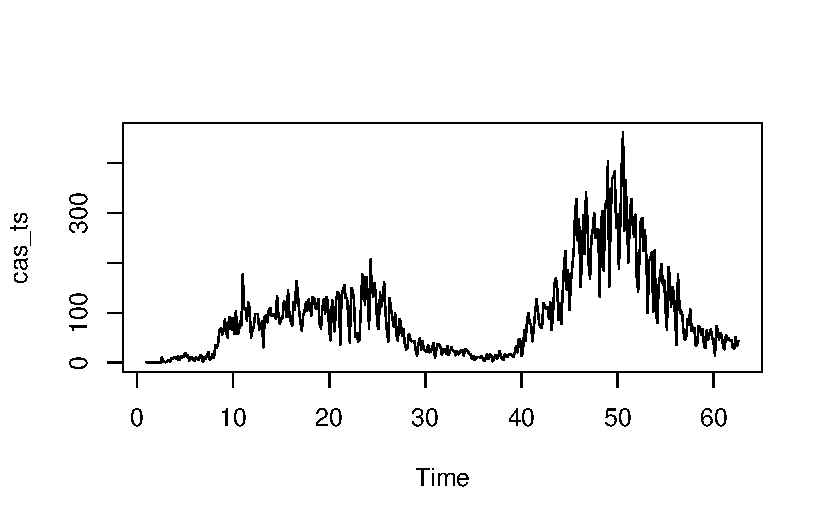
\includegraphics{TS_files/figure-pdf/unnamed-chunk-1-1.pdf}

\subsection{2. Décomposition et analyse de la
tendance}\label{duxe9composition-et-analyse-de-la-tendance}

\begin{Shaded}
\begin{Highlighting}[]
\CommentTok{\# Décomposer la série avec une saisonnalité hebdomadaire (fréquence =7)}

\NormalTok{decomposition }\OtherTok{\textless{}{-}} \FunctionTok{stl}\NormalTok{(cas\_ts, }\AttributeTok{s.window=}\StringTok{"periodic"}\NormalTok{)}
\FunctionTok{plot}\NormalTok{(decomposition)}
\end{Highlighting}
\end{Shaded}

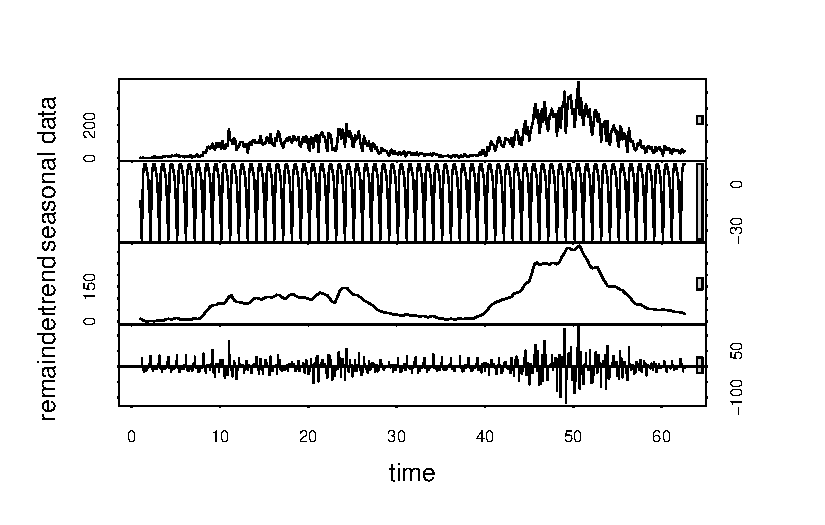
\includegraphics{TS_files/figure-pdf/unnamed-chunk-2-1.pdf}

\paragraph{Interprétation}\label{interpruxe9tation}

\begin{itemize}
\item
  \textbf{Tendance} : La tendance représente la direction générale de
  l'évolution des cas positifs. Elle montre une montée et une baisse au
  fil du temps, permettant d'identifier les phases critiques de la
  pandémie.
\item
  \textbf{Saisonnalité} : La saisonnalité détecte des fluctuations
  répétitives hebdomadaires, probablement liées à des variations des
  tests effectués selon les jours de la semaine (moins de tests le
  week-end, par exemple).
\item
  \textbf{Résidus} : Les résidus représentent les variations non
  expliquées par la tendance et la saisonnalité. Ils devraient
  idéalement être aléatoires (bruit blanc), mais des résidus importants
  peuvent indiquer des événements imprévus ou des changements de
  comportement non capturés par les autres composantes.\\
  \strut \\
\end{itemize}

\subsubsection{3. Moyenne mobile et tendance
linéaire}\label{moyenne-mobile-et-tendance-linuxe9aire}

\begin{Shaded}
\begin{Highlighting}[]
\CommentTok{\# Calcul de la moyenne mobile}
\NormalTok{mm\_7 }\OtherTok{\textless{}{-}} \FunctionTok{ma}\NormalTok{(cas\_ts, }\AttributeTok{order=}\DecValTok{7}\NormalTok{)}

\CommentTok{\# Visualisation avec moyenne mobile}
\FunctionTok{plot}\NormalTok{(cas\_ts, }\AttributeTok{main=}\StringTok{"Cas Positifs avec Moyenne Mobile"}\NormalTok{, }
     \AttributeTok{ylab=}\StringTok{"Nombre de cas"}\NormalTok{, }\AttributeTok{xlab=}\StringTok{"Temps"}\NormalTok{)}
\FunctionTok{lines}\NormalTok{(mm\_7, }\AttributeTok{col=}\StringTok{"red"}\NormalTok{, }\AttributeTok{lwd=}\DecValTok{2}\NormalTok{)}

\CommentTok{\# Ajout de la tendance linéaire}
\NormalTok{temps }\OtherTok{\textless{}{-}} \DecValTok{1}\SpecialCharTok{:}\FunctionTok{length}\NormalTok{(cas\_ts)}
\NormalTok{modele\_lineaire }\OtherTok{\textless{}{-}} \FunctionTok{lm}\NormalTok{(}\FunctionTok{as.vector}\NormalTok{(cas\_ts) }\SpecialCharTok{\textasciitilde{}}\NormalTok{ temps)}
\FunctionTok{lines}\NormalTok{(temps, }\FunctionTok{predict}\NormalTok{(modele\_lineaire), }\AttributeTok{col=}\StringTok{"blue"}\NormalTok{, }\AttributeTok{lwd=}\DecValTok{2}\NormalTok{)}
\FunctionTok{legend}\NormalTok{(}\StringTok{"topleft"}\NormalTok{, }\AttributeTok{legend=}\FunctionTok{c}\NormalTok{(}\StringTok{"Données brutes"}\NormalTok{, }\StringTok{"Moyenne mobile"}\NormalTok{, }\StringTok{"Tendance linéaire"}\NormalTok{), }
       \AttributeTok{col=}\FunctionTok{c}\NormalTok{(}\StringTok{"black"}\NormalTok{, }\StringTok{"red"}\NormalTok{, }\StringTok{"blue"}\NormalTok{), }\AttributeTok{lty=}\DecValTok{1}\NormalTok{)}
\end{Highlighting}
\end{Shaded}

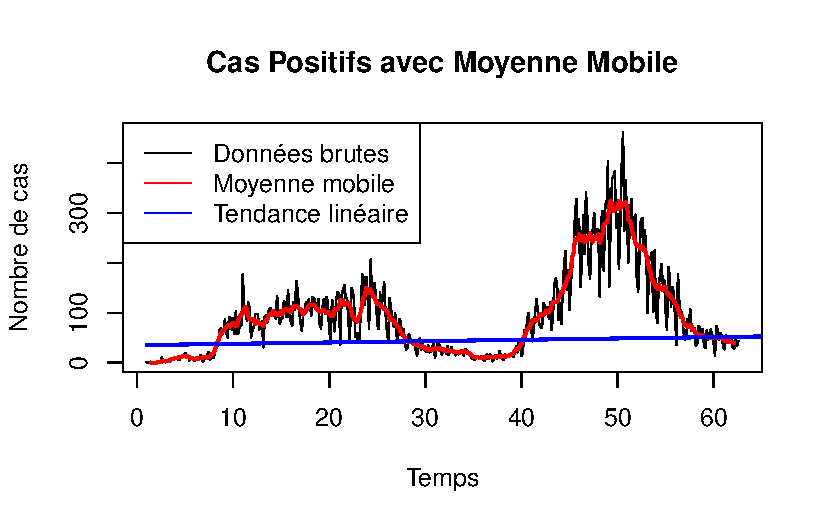
\includegraphics{TS_files/figure-pdf/unnamed-chunk-3-1.pdf}

\paragraph{\texorpdfstring{\textbf{Interprétation}}{Interprétation}}\label{interpruxe9tation-1}

La courbe de la moyenne mobile sur 7 jours lisse les fluctuations
quotidiennes et montre une tendance plus claire. On voit ici que, malgré
les fluctuations journalières, la tendance générale peut être identifiée
à travers cette moyenne mobile.

\subsection{4. Modélisation
Box-Jenkins}\label{moduxe9lisation-box-jenkins}

\subsubsection{Tests de stationnarité}\label{tests-de-stationnarituxe9}

\begin{Shaded}
\begin{Highlighting}[]
\CommentTok{\# Test sur série originale}
\NormalTok{adf\_test }\OtherTok{\textless{}{-}} \FunctionTok{adf.test}\NormalTok{(cas\_ts)}
\FunctionTok{print}\NormalTok{(}\StringTok{"Test ADF sur série originale :"}\NormalTok{)}
\end{Highlighting}
\end{Shaded}

\begin{verbatim}
[1] "Test ADF sur série originale :"
\end{verbatim}

\begin{Shaded}
\begin{Highlighting}[]
\FunctionTok{print}\NormalTok{(adf\_test)}
\end{Highlighting}
\end{Shaded}

\begin{verbatim}

    Augmented Dickey-Fuller Test

data:  cas_ts
Dickey-Fuller = -0.70951, Lag order = 7, p-value = 0.9694
alternative hypothesis: stationary
\end{verbatim}

\begin{Shaded}
\begin{Highlighting}[]
\CommentTok{\# Test sur série différenciée}
\NormalTok{cas\_diff }\OtherTok{\textless{}{-}} \FunctionTok{diff}\NormalTok{(cas\_ts)}
\NormalTok{adf\_test\_diff }\OtherTok{\textless{}{-}} \FunctionTok{adf.test}\NormalTok{(cas\_diff)}
\FunctionTok{print}\NormalTok{(}\StringTok{"Test ADF sur série différenciée :"}\NormalTok{)}
\end{Highlighting}
\end{Shaded}

\begin{verbatim}
[1] "Test ADF sur série différenciée :"
\end{verbatim}

\begin{Shaded}
\begin{Highlighting}[]
\FunctionTok{print}\NormalTok{(adf\_test\_diff)}
\end{Highlighting}
\end{Shaded}

\begin{verbatim}

    Augmented Dickey-Fuller Test

data:  cas_diff
Dickey-Fuller = -9.0383, Lag order = 7, p-value = 0.01
alternative hypothesis: stationary
\end{verbatim}

\paragraph{Interprétation}\label{interpruxe9tation-2}

\begin{itemize}
\item
  Sur la série originale, p-value = 0.97 \textgreater{} 0.05, série non
  stationnaire
\item
  Sur la série différenciée, p-value = 0.01 \textless{} 0.05, série
  stationnaire
\end{itemize}

\subsubsection{5. Analyse ACF et PACF}\label{analyse-acf-et-pacf}

\begin{Shaded}
\begin{Highlighting}[]
\FunctionTok{par}\NormalTok{(}\AttributeTok{mfrow=}\FunctionTok{c}\NormalTok{(}\DecValTok{2}\NormalTok{,}\DecValTok{1}\NormalTok{))}
\FunctionTok{par}\NormalTok{(}\AttributeTok{mar=}\FunctionTok{c}\NormalTok{(}\DecValTok{4}\NormalTok{,}\DecValTok{4}\NormalTok{,}\DecValTok{2}\NormalTok{,}\DecValTok{2}\NormalTok{))}
\FunctionTok{acf}\NormalTok{(cas\_diff, }\AttributeTok{main=}\StringTok{"ACF des différences premières"}\NormalTok{)}
\FunctionTok{pacf}\NormalTok{(cas\_diff, }\AttributeTok{main=}\StringTok{"PACF des différences premières"}\NormalTok{)}
\end{Highlighting}
\end{Shaded}

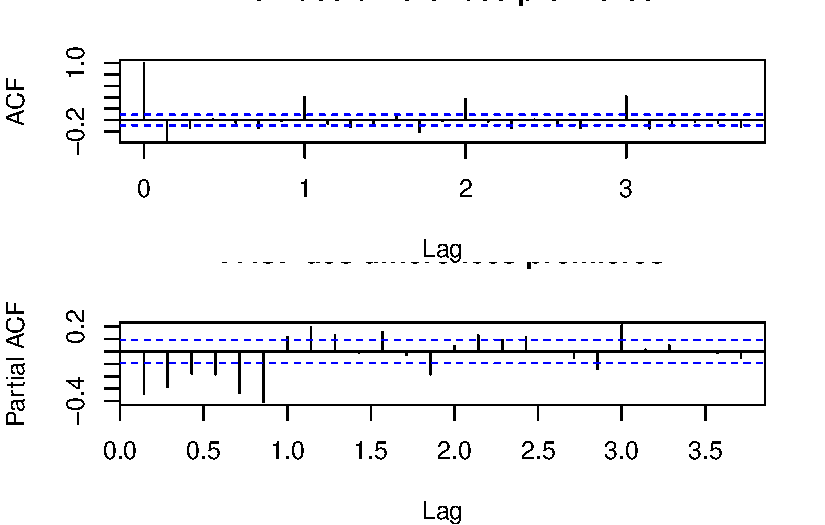
\includegraphics{TS_files/figure-pdf/unnamed-chunk-5-1.pdf}

\paragraph{Interprétation}\label{interpruxe9tation-3}

\subsubsection{1. ACF (Autocorrelation
Function)}\label{acf-autocorrelation-function}

\begin{itemize}
\tightlist
\item
  On observe que toutes les valeurs sont proches de zéro, avec quelques
  barres dépassant légèrement les intervalles de confiance, il n'y a pas
  de corrélations significatives dans les données différenciées, ce qui
  est souvent un signe que la série différenciée est
  \textbf{stationnaire}.
\end{itemize}

\subsubsection{2. PACF (Partial Autocorrelation
Function)}\label{pacf-partial-autocorrelation-function}

\begin{itemize}
\tightlist
\item
  Ici, la première barre est significative, tandis que les suivantes
  sont proches de zéro, à l'intérieur des intervalles de confiance.\\
  \strut \\
\end{itemize}

\subsubsection{6. Modélisation ARIMA}\label{moduxe9lisation-arima}

\begin{Shaded}
\begin{Highlighting}[]
\NormalTok{modele\_auto }\OtherTok{\textless{}{-}} \FunctionTok{auto.arima}\NormalTok{(cas\_diff, }\AttributeTok{seasonal=}\ConstantTok{TRUE}\NormalTok{)}
\FunctionTok{summary}\NormalTok{(modele\_auto)}
\end{Highlighting}
\end{Shaded}

\begin{verbatim}
Series: cas_diff 
ARIMA(0,0,1)(1,0,1)[7] with zero mean 

Coefficients:
          ma1    sar1     sma1
      -0.7391  0.8982  -0.6020
s.e.   0.0321  0.0284   0.0529

sigma^2 = 962.1:  log likelihood = -2092.59
AIC=4193.18   AICc=4193.27   BIC=4209.44

Training set error measures:
                      ME     RMSE      MAE MPE MAPE      MASE         ACF1
Training set -0.05961689 30.90945 20.50475 NaN  Inf 0.6203363 -0.006537767
\end{verbatim}

\paragraph{Interprétation}\label{interpruxe9tation-4}

Le modèle ARIMA sélectionné automatiquement est
\textbf{ARIMA(0,0,1)(1,0,1){[}7{]}} avec zéro moyenne. Cela signifie :

\begin{itemize}
\item
  p = 0 p = 0 p = 0 : pas de termes autoregressifs.
\item
  d = 0 d = 0 d = 0 : pas de différenciation.
\item
  q = 1 q = 1 q = 1 : un terme de moyenne mobile.
\item
  Une composante saisonnière avec P=1 P= 1 P= 1, Q= 1 Q =1 Q= 1 et une
  fréquence de 7 (hebdomadaire).
\end{itemize}

Les coefficients du modèle montrent des relations significatives, et
l'erreur quadratique moyenne (RMSE) est de \textbf{30.91} sur l'ensemble
d'entraînement.

\subsection{7. Prévisions}\label{pruxe9visions}

\subsubsection{7.1 Prévisions ARIMA sur 30
jours}\label{pruxe9visions-arima-sur-30-jours}

\begin{Shaded}
\begin{Highlighting}[]
\CommentTok{\# Prévisions ARIMA}
\NormalTok{prev\_arima }\OtherTok{\textless{}{-}} \FunctionTok{forecast}\NormalTok{(modele\_auto, }\AttributeTok{h=}\DecValTok{30}\NormalTok{)}
\FunctionTok{plot}\NormalTok{(prev\_arima, }\AttributeTok{main=}\StringTok{"Prévisions ARIMA sur 30 jours"}\NormalTok{,}
     \AttributeTok{xlab=}\StringTok{"Temps"}\NormalTok{, }\AttributeTok{ylab=}\StringTok{"Nombre de cas positifs"}\NormalTok{)}
\end{Highlighting}
\end{Shaded}

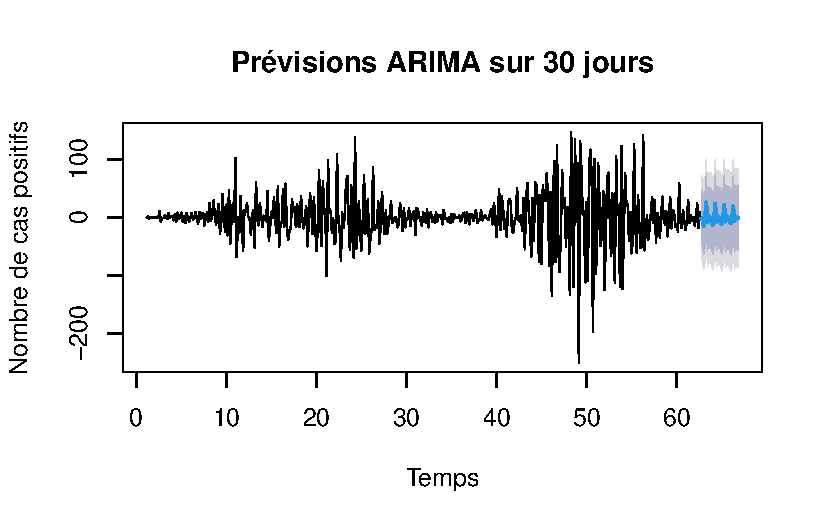
\includegraphics{TS_files/figure-pdf/unnamed-chunk-7-1.pdf}

\paragraph{Interprétation}\label{interpruxe9tation-5}

Les prévisions ARIMA montrent l'évolution des cas positifs sur les 30
jours suivants, avec des bandes de confiance. Ces bandes deviennent plus
larges au fil du temps, indiquant une incertitude croissante dans les
prévisions à mesure que l'horizon de prévision s'allonge.

\begin{center}\rule{0.5\linewidth}{0.5pt}\end{center}

\begin{center}\rule{0.5\linewidth}{0.5pt}\end{center}

\subsubsection{7.2 Prévisions par LISSAGE EXPONENTIEL ETS (Error, Trend,
Seasonality) sur 30
jours}\label{pruxe9visions-par-lissage-exponentiel-ets-error-trend-seasonality-sur-30-jours}

\begin{Shaded}
\begin{Highlighting}[]
\CommentTok{\# Modèle ETS}
\NormalTok{modele\_ets }\OtherTok{\textless{}{-}} \FunctionTok{ets}\NormalTok{(cas\_ts)}
\NormalTok{prev\_ets }\OtherTok{\textless{}{-}} \FunctionTok{forecast}\NormalTok{(modele\_ets, }\AttributeTok{h=}\DecValTok{30}\NormalTok{)}

\CommentTok{\# Préparation des données pour la comparaison}
\NormalTok{df\_comparaison }\OtherTok{\textless{}{-}} \FunctionTok{data.frame}\NormalTok{(}
    \AttributeTok{Date =} \DecValTok{1}\SpecialCharTok{:}\DecValTok{30}\NormalTok{,}
    \AttributeTok{ARIMA =} \FunctionTok{as.numeric}\NormalTok{(prev\_arima}\SpecialCharTok{$}\NormalTok{mean),}
    \AttributeTok{ETS =} \FunctionTok{as.numeric}\NormalTok{(prev\_ets}\SpecialCharTok{$}\NormalTok{mean)}
\NormalTok{)}

\NormalTok{df\_long }\OtherTok{\textless{}{-}} \FunctionTok{pivot\_longer}\NormalTok{(df\_comparaison, }
                       \AttributeTok{cols =} \FunctionTok{c}\NormalTok{(}\StringTok{"ARIMA"}\NormalTok{, }\StringTok{"ETS"}\NormalTok{),}
                       \AttributeTok{names\_to =} \StringTok{"Methode"}\NormalTok{, }
                       \AttributeTok{values\_to =} \StringTok{"Prevision"}\NormalTok{)}

\CommentTok{\# Visualisation comparative}
\FunctionTok{ggplot}\NormalTok{(df\_long, }\FunctionTok{aes}\NormalTok{(}\AttributeTok{x =}\NormalTok{ Date, }\AttributeTok{y =}\NormalTok{ Prevision, }\AttributeTok{color =}\NormalTok{ Methode)) }\SpecialCharTok{+}
    \FunctionTok{geom\_line}\NormalTok{() }\SpecialCharTok{+}
    \FunctionTok{labs}\NormalTok{(}\AttributeTok{title =} \StringTok{"Comparaison des prévisions ARIMA et ETS"}\NormalTok{,}
         \AttributeTok{x =} \StringTok{"Jours de prévision"}\NormalTok{,}
         \AttributeTok{y =} \StringTok{"Nombre de cas positifs"}\NormalTok{) }\SpecialCharTok{+}
    \FunctionTok{theme\_minimal}\NormalTok{()}
\end{Highlighting}
\end{Shaded}

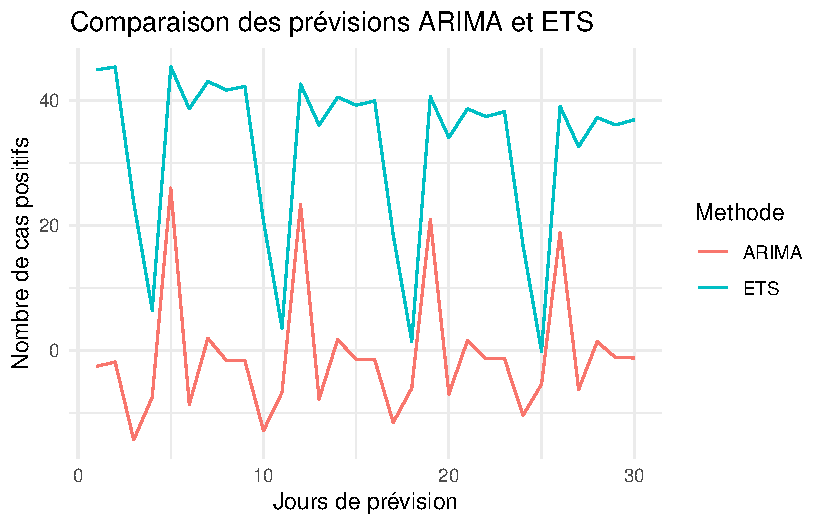
\includegraphics{TS_files/figure-pdf/unnamed-chunk-8-1.pdf}

\paragraph{Interprétation}\label{interpruxe9tation-6}

\begin{itemize}
\item
  Le modèle ETS, qui prend en compte les composantes d'erreur, de
  tendance et de saisonnalité, fournit également des prévisions sur 30
  jours. Il est souvent plus flexible pour des données saisonnières ou
  avec une tendance non linéaire.
\item
  La comparaison graphique des prévisions ARIMA et ETS montre des
  différences potentielles dans la manière dont les deux modèles
  anticipent l'évolution des cas. Il est important de noter que chaque
  modèle peut mieux capturer certains aspects des données (ARIMA pour la
  dynamique temporelle autoregressive et ETS pour la détection des
  tendances/saisons complexes).
\end{itemize}

\begin{center}\rule{0.5\linewidth}{0.5pt}\end{center}

\begin{center}\rule{0.5\linewidth}{0.5pt}\end{center}

\begin{center}\rule{0.5\linewidth}{0.5pt}\end{center}

\subsubsection{8. Évaluation de la précision des
modèles}\label{uxe9valuation-de-la-pruxe9cision-des-moduxe8les}

\begin{Shaded}
\begin{Highlighting}[]
\FunctionTok{print}\NormalTok{(}\StringTok{"Précision du modèle ARIMA :"}\NormalTok{)}
\end{Highlighting}
\end{Shaded}

\begin{verbatim}
[1] "Précision du modèle ARIMA :"
\end{verbatim}

\begin{Shaded}
\begin{Highlighting}[]
\FunctionTok{accuracy}\NormalTok{(prev\_arima)}
\end{Highlighting}
\end{Shaded}

\begin{verbatim}
                      ME     RMSE      MAE MPE MAPE      MASE         ACF1
Training set -0.05961689 30.90945 20.50475 NaN  Inf 0.6203363 -0.006537767
\end{verbatim}

\begin{Shaded}
\begin{Highlighting}[]
\FunctionTok{print}\NormalTok{(}\StringTok{"Précision du modèle ETS :"}\NormalTok{)}
\end{Highlighting}
\end{Shaded}

\begin{verbatim}
[1] "Précision du modèle ETS :"
\end{verbatim}

\begin{Shaded}
\begin{Highlighting}[]
\FunctionTok{accuracy}\NormalTok{(prev\_ets)}
\end{Highlighting}
\end{Shaded}

\begin{verbatim}
                    ME     RMSE      MAE MPE MAPE      MASE       ACF1
Training set 0.2317715 31.35175 21.72128 NaN  Inf 0.8129221 0.03148064
\end{verbatim}

\paragraph{Interprétation}\label{interpruxe9tation-7}

\begin{itemize}
\item
  \textbf{ARIMA} : Le RMSE (Root Mean Square Error) est de
  \textbf{30.91} et le MAE (Mean Absolute Error) de \textbf{20.50}. Cela
  signifie que le modèle ARIMA a une erreur moyenne relativement faible.
\item
  \textbf{ETS} : Le RMSE est de \textbf{31.35} et le MAE de
  \textbf{21.72}. Légèrement plus élevé que celui du modèle ARIMA,
  indiquant que le modèle ETS est un peu moins précis que l'ARIMA pour
  cette série temporelle spécifique.
\item
  \textbf{Performance Comparée} : Dans l'ensemble, le modèle
  \textbf{ARIMA} semble avoir une meilleure précision que le modèle
  \textbf{ETS} en raison de son RMSE et MAE inférieurs, ce qui suggère
  qu'il pourrait être préférable pour ces données spécifiques.
\end{itemize}



\end{document}
